\section{Оборудование}

Экспериментальная установка состоит из стеклянного сосуда А, снабженного краном К1 и
U-образного жидкостного манометра, измеряющего избыточное давление газа в сосуде.
Схема установки показана на рисунке (вместо груши используется сосуд с углекислым газом).
\begin{figure}[ht!]
    \centering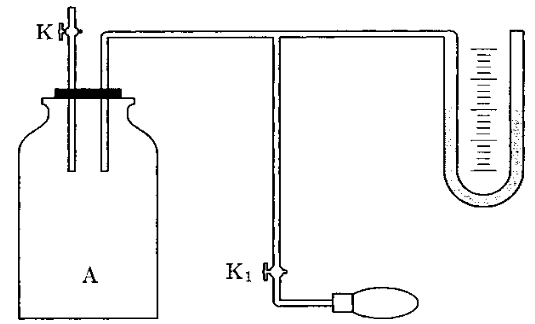
\includegraphics[width=0.8\linewidth]{img/img1.png}
\end{figure}

Проведем с установкой следующие манипуляции:
\begin{enumerate}
    \item Закроем кран К2 (0)
    \item Откроем кран К1 на некоторое время
    \item Закроем кран К1 (1)
    \item Дождемся установления равновесия (2)
    \item Откроем кран К2 на некоторое время $\tau$ (3)
    \item Дождемся установления равновесия (4)
    \item Откроем кран К2 (5)
    \item Подождем 3-4 минуты (0)
\end{enumerate}

В результате некоторая порция газа совершает процесс, показанный на рисунке.
\begin{figure}[ht!]
    \centering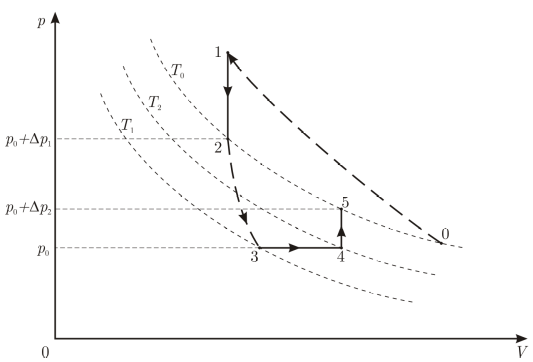
\includegraphics[width=0.8\linewidth]{img/img2.png}
\end{figure}

В сосуде создается избыточное давление $p_1$. При втечении в систему газ оказывается нагретым.

Мысленно выделим в сосуде объем $\Delta V$ газа. Будем следить за изменением его состояния.
Вследствие теплообмена со стенками сосуда через некоторое время газ остынет до комнатной температуры
$T_0$ (процесс 12). При этом давление понизится до $p_0 + \Delta p_1$
\[\Delta p_1 = \rho g\Delta h_1\]

После открытия К2 за время порядка $0{,}5\,\text{с}$ произойдет адиабатическое расширение
и его температура окажется ниже комнатной. Далее газ будет изобарически нагреваться (процесс 34).
Зададим время $\tau$, в течение которого кран К2 остается открытым таким, чтобы можно было
пренебречь временем $\Delta t$ адиабатического расширения воздуха. После закрытия крана К2
газ станет изохорически нагреваться до комнатной температуры (процесс 45), причем давление
внутри возрастет до $p_0 + \Delta p_2$, где 
\[\Delta p_2 = \rho g\Delta h_2\] 

Наибольший интерес представляет исследование зависимости отношения перепадов давления
$\frac{\Delta p_1}{\Delta p_2}$ от времени $\tau$.

С хорошей точностью мы можем считать воздух в газгольдере идеальным газом.
Рассмотрим изобарическое расширение воздуха. Для этого запишем уравнение теплового баланса
для изменяющейся со временем массы газа $m=\frac{p_0V_0}{RT}\mu$:
\[c_pm\,dT=-\alpha(T-T_0)\,dt,\]
где $c_p$ --- удельная теплоёмкость воздуха при постоянном давлении, $\alpha$ ---
положительный постоянный коэффициент, характеризующий теплообмен, $V_0$ --- объем газгольдера.

\[c_p\frac{p_0V_0}{RT}\mu\,dT = -\alpha (T-T_0)\,dt\]
\[\frac{1}{T(T-T_0)}=-\frac{1}{T_0}\left(\frac{1}{T}-\frac{1}{T-T_0}\right)\]
Тогда
\[\frac{1}{T_0}\left(\frac{1}{T} - \frac{1}{T-T_0}\right)\, dT = \frac{\alpha\, dt}{c_pm_0T_0}\]

\[\ln\frac{T_2}{T_1} - \ln\frac{T_2-T_0}{T_1-T_0}=\frac{\alpha}{c_pm_0}\tau\]
\[\frac{\Delta T_1}{T_1} = \frac{\Delta T_2}{T_2}\exp\left(\frac{\alpha}{c_pm_0}\tau\right)\]

Для адиабатического расширения $T^\gamma = \mathrm{const}\,p^{\gamma-1}$
\[\frac{dT}{T}=\frac{\gamma-1}{\gamma}\frac{dp}{p}\]
\[\frac{\Delta T_1}{T_1}=\frac{\gamma-1}{\gamma}\frac{\Delta p_1}{p_0}\]

При изохорическом нагреве газа выполняется соотношение $\frac{p}{T}=\mathrm{const}$.
\[\frac{\Delta T_2}{T_2}=\frac{\Delta p_2}{p_0}\]
\[\frac{\gamma-1}{\gamma}\frac{\Delta p_1}{p_0} = \frac{\Delta p_2}{p_0}\exp\left(\frac{\alpha}{c_pm_0}\tau\right)\]
\[\frac{\gamma-1}{\gamma}\Delta h_1 = \Delta h_2\exp\left(\frac{\alpha}{c_pm_0}\tau\right)\]
\[\ln\frac{\Delta h_1}{\Delta h_2} = \ln\frac{\gamma}{\gamma-1} + \frac{\alpha}{c_pm_0}\tau\]

Из графика зависимости $\ln\frac{\Delta h_1}{\Delta h_2}$ от $\tau$ определим $\gamma$.

